\section{Auswertung}
\label{sec:Auswertung}

\subsection{statische Methode}
In diesem Kapitel werden die Unterschiede und Gemeinsamkeiten der vier 
Temperaturverläufe $T1$, $T4$, $T5$, $T8$ zu den unterschiedlichen Materialien 
ausgewertet. Weiterhin wird der Stab mit der besten Wärmeleitung bestimmt und 
der Wärmestrom zu jeder Messzeit. Letztlich werden noch die Temperaturdifferenzen 
$\Delta T_{ST}=T7-T8$ und $T_{ST}=T2-T1$ als Funktionen der Messzeit t dargestellt.

\subsubsection{Temperaturverläufe und Wärmeleitung}
\begin{figure}[H]
    \centering
    \includegraphics[width=\textwidth]{tempverlaufT1T4.pdf}
    \caption{Temperaturverläufe von $T1$ und $T4$.}
    \label{fig:f1}
\end{figure}
Bei den beiden Stäben aus \autoref{fig:f1} handelt es sich um Messingstäbe. Der 
Temperaturverlauf verhält sich demnach ziemlich ähnlich. Die Abweichung zwischen 
beiden Verläufen ist mit dem Flächenunterschied zu begründen; die Stäbe von 
T1 und T4 sind unterschiedlicher Größe und da nach \autoref{eqn:1} die Fläche
$A$ proportional zu der Wärmemenge $dQ$ ist, weist T1 eine etwas höhere Temperatur 
auf. Die Abweichung nach oben ist mit einem Messfehler verbunden, welcher noch 
zu diskutieren ist.
\\
In \autoref{fig:f2} befindt sich der Temperaturverlauf des Aluminiumstabs(T5)
und des Edelstahlstabs(T8).
\begin{figure}[H]
    \centering
    \includegraphics[width=\textwidth]{tempverlaufT5T8.pdf}
    \caption{Temperaturverläufe von $T5$ und $T8$.}
    \label{fig:f2}
\end{figure}
\noindent Es ist zunächst zu erkennen, dass der Temperaturverlauf des
Aluminiumstabs recht stark von dem des Edelstahlstabs abweicht. Dieser Verlauf
lässt sich mit der höheren Wärmeleitfähigkeit des Aluminiums erklären. Im 
Vergleich mit den anderen Werten zum Zeitpunkt $t$ = 700s:
\begin{center}
  $T1$ = 43,65°C\\
  $T4$ = 41,41°C\\
  $T5$ = 46,24°C\\
  $T8$ = 33,62°C
\end{center}
Der Aluminiumstab verfügt demnach offenbar über die stärkste Wärmeleitfähigkeit.
Nun lässt sich der Wärmestrom berechnen, indem \autoref{eqn:1} umgeformt wird nach:
\begin{equation}
  \frac{\Delta Q}{\Delta t} = - \kappa A \frac{\partial T}{\partial x}
\end{equation}
Dabei ist $\partial T = T_i - T_j$ und $\partial x$ die ausgemessene Größe von 
0,03m.

In folgender Tabelle wird der Wärmestrom zu 5 unterschiedlichen Zeiten dargestellt.
$\Delta Q_{T1-T2}$ steht für den Wärmestrom zwischen $T1$ und $T2$, analog ergibt 
sich der Wärmestrom $\Delta Q_{T8-T7}$ zwischen den Thermoelementen $T7$ und $T8$.
\begin{table}[H]
  \centering
  \caption{Wärmestrom für 5 Zeiten}
  \label{tab:t1}
  %\sisetup{table-format=1.1, per-mode=reciprocal}
  \begin{tblr}{
      colspec = {S S S},
      row{1} = {guard, mode=math},
      %vline{4} = {2}{-}{text=\clap{$\pm$}},
    }
    \toprule
    % t/s & $\Delta Q_{T1-T2}/ \Delta t$ & $\Delta Q_{T8-T7}/ \Delta t$\\
    t/s & \frac{\Delta Q_{T1-T2}}{\Delta t}/W & \frac{\Delta Q_{T8-T7}}{\Delta t}/W \\
    \midrule
    100 & -0,62 & -0,97 \\
    200 & -0,35 & -0,88 \\
    400 & -0,21 & -0,71 \\
    600 & -0,11 & -0,64 \\
    800 & -0,24 & -0,77 \\
    \bottomrule
  \end{tblr}
\end{table}

\subsubsection{Temperaturdifferenz}
In \autoref{fig:f3} ist die Temperaturdifferenz der ersten beiden Thermoelemente 
zu sehen.
\begin{figure}[H]
  \centering
  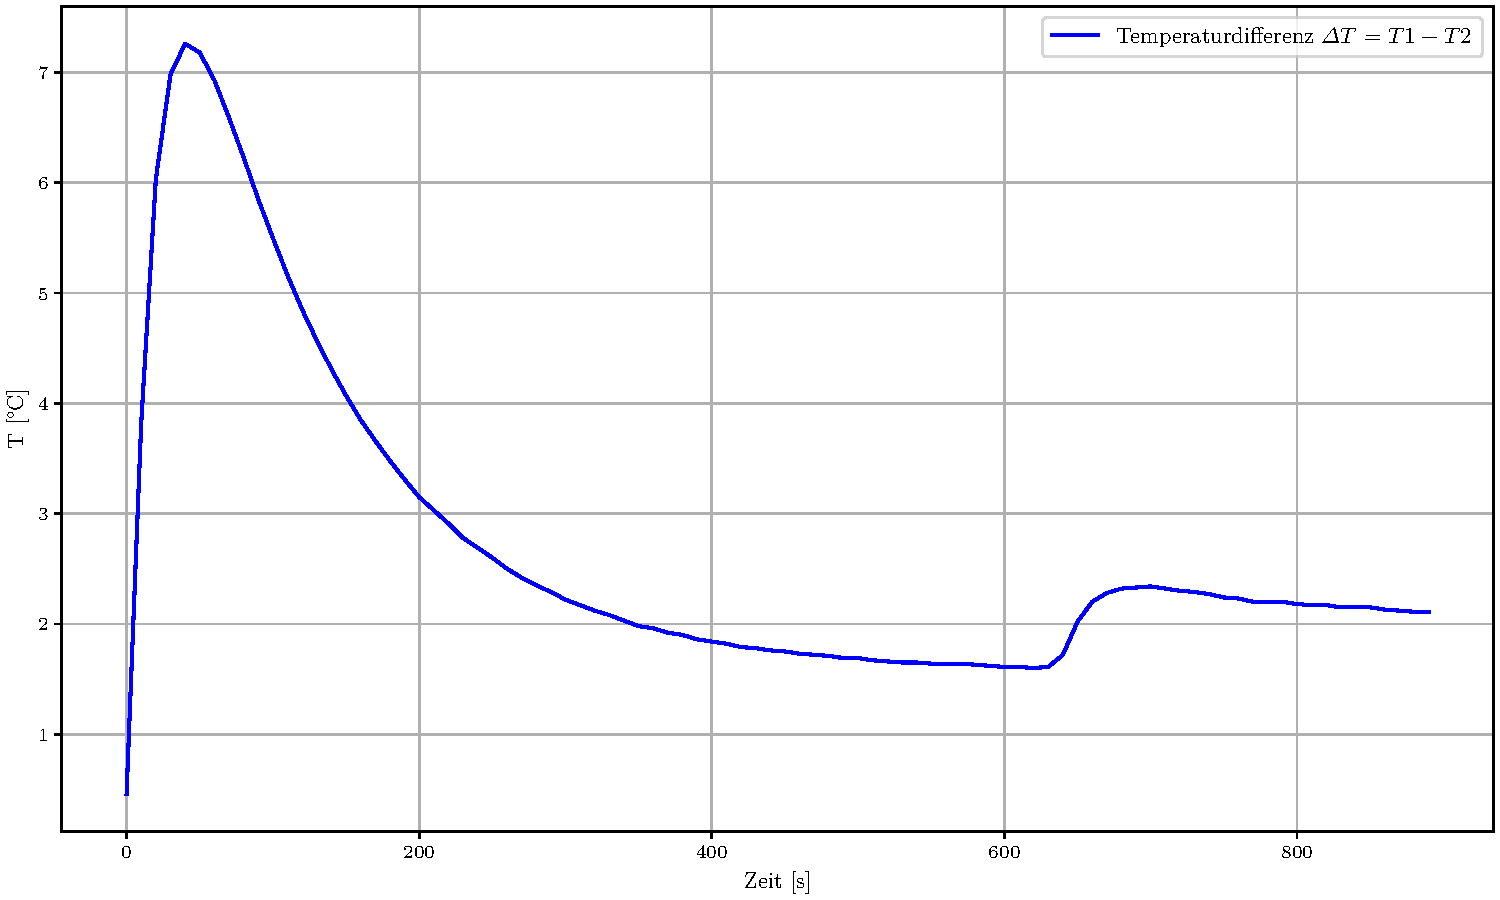
\includegraphics[width=\textwidth]{plotdiff12.pdf}
  \caption{Temperaturdifferenz $T1$ und $T2$.}
  \label{fig:f3}
\end{figure}
\noindent In folgender Abbildung befindet sich die Differenz der letzten beiden Thermoelemente.
Dabei fällt auf, dass sich die zeitlichen Entwicklungen ähneln; nach Erreichen 
einer Maximaltemperatur fällt der Graph asymptotisch, wobei der Graph aus 
\autoref{fig:f4} temperaturmäßig weiter oben liegt und nicht so stark sinkt, wie 
der Graph aus \autoref{fig:f3}, was durch die bessere Wärmeleitfähigkeit des Messings 
im Gegensatz zum Edelstahl zu begründen ist. Die erste maximale
Temperaturdifferenz liegt dabei bei etwa 7,3°C und beim Zweiten Graphen bei 
knapp 12,1°C. Auffällig bei beiden Graphen ist wieder der Messfehler am rechten
Ende des Graphen. Dieser wird in der Diskussion behandelt. 
\begin{figure}[H]
  \centering
  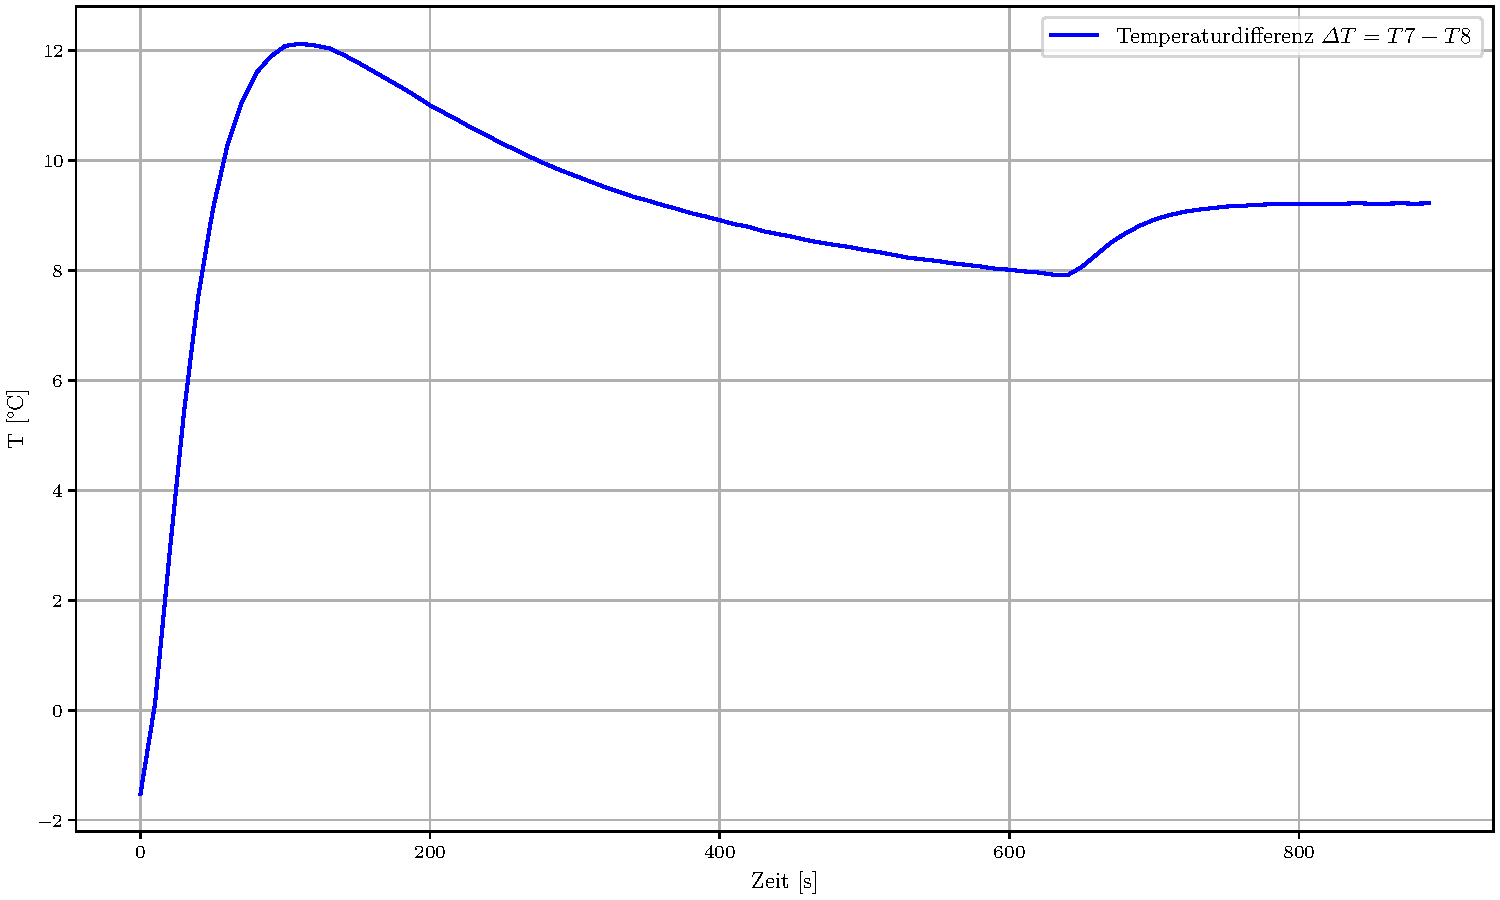
\includegraphics[width=\textwidth]{plotdiff78.pdf}
  \caption{Temperaturdifferenz $T7$ und $T8$.}
  \label{fig:f4}
\end{figure}



\subsection{Dynamische Methode}
Hier wird die Wärmeleitfähigkeit für den breiten Messingstab, den Aluminiumstab und den Elelstahlstab
mithilfe der in der \autoref{sec:Auswertung} erwähnten dynamischen Methode ermittelt.
\subsubsection{Wärmeleitfähigkeit Messing}
Zur Berechnung der Wärmeleitfähigkeit von Messing werden die Messwerte des breiten Messsingstabes
mit den Temperaturmesselementen $T_1$ und $T_2$ benutzt. Jene Wärmeleitfähigkeit lässt sich mit
\autoref{eqn:6} bestimmen. Darin sind $\Delta x = 0.03\unit{\meter}$ der Abstand der Temperaturmesselemente, $c$ die Materialabhängige
Wärmekapazität, $\rho $ die Dichte des Stabes, $\Delta t$ die Phasendifferenz
zwischen der Temperaturwelle am ersten und zweiten Temperaturelement und $A_{nah/fern}$
die Amplituden der jeweiligen Temperaturwelle. Die Minima und Maxima werden
durch die Funktion "find$\_$peaks " , aus der Bibiliothek SciPy, bestimmt. Daraus
lassen sich  mithilfe von \autoref{eqn:A} die Amplituden berechnen.

\begin{equation}
  \label{eqn:A}
  A_{pos} = \frac{1}{2}\left(A_{max,i+1}-\frac{1}{2}\left(A_{min,i-1}-A_{min,i}\right)-A_{min}\right)
\end{equation}

\begin{table}[H]
  \centering
  \caption{Ermittelte Amplituden und Phasendifferenz für Messing.}
  \label{tab:t2}
  %\sisetup{table-format=1.1, per-mode=reciprocal}
  \begin{tblr}{
      colspec = {S S S S},
      row{1} = {guard, mode=math},
    }
    \toprule
    A_{fern} & A_{nah} & \ln{\frac{A_{nah}}{A_{fern}}} & \Delta t \unit{\second}\\
    \midrule
    1.00  &1.91  &0.648 &28\\
    0.89  &1.87  &0.734 &20\\
    0.72  &1.69  &0.847 &18\\
    0.77  &1.83  &0.863 &14\\
    0.60  &1.59  &0.966 &14\\
    0.62  &1.63  &0.956 &14\\
    0.57  &1.60  &1.020 &12\\
    0.48  &1.50  &1.144 &14\\
    0.52  &1.52  &1.066 &12\\
    0.52  &1.52  &1.059 &12\\
    \bottomrule
  \end{tblr}
\end{table}
\noindent In \autoref{tab:t2} sind die durch \autoref{eqn:A} ermittelten 
Amplituden, sowie der Logarithmus dieser und die Phasendifferenz 
$\Delta t$ aufgeführt. Des Weiteren sind in \autoref{fig:mp} die Messwerte 
mit den ermittelten Hoch-und Tiefpunkte grafisch dargestellt.

\begin{figure}[H]
  \centering
  \caption{Graphische Darstellung der gemessenen Temperaturen $T_1$ und $T_2$ pro vergangenen zwei Sekunden.}
  \label{fig:mp}
  \includegraphics{messingPlot}
\end{figure}

\noindent Zusammen mit den Materialeigenschaften $\rho$ und $c$, dem Abstand 
$\Delta x$, sowie den gemittelten Größen $\Delta t $ und 
$ \ln{\frac{A_{nah}}{A_{fern}}}$ aus den im Vorherigen ermittelten Größen,
lässt sich die Wärmeleitfähigkeit von Messing über \autoref{eqn:6} bestimmen.
Der fehler des Mittelwertes lässt sich über \autoref{eqn:7} berechnen.
\begin{align*}
  \rho_{Messing}                                &= \qty{8520}{\kilo\gram\per\cubic\meter}\\
  \Delta x                              &= \qty{0.03}{\meter}\\
  c_{Messing}                                   &= \qty{385}{\joule\per\kilo\gram\kelvin}\\
  \overline{\ln{\frac{A_{nah}}{A_{fern}}}}  &= \qty{0.93(0.04)}{}\\
  \overline{\Delta t}                   &= \qty{15.45(1.4)}{\second}
\end{align*}

\noindent Die Berechnung der Wärmekapazität ergibt nach Einsetzen der Werte:
\begin{equation}
  \kappa_{Messing} = \qty{103(11)}{\watt\per\meter\kelvin}
\end{equation}

\subsubsection{Wärmeleitfähigkeit Aluminium}
Auch für Aluminium wird die Wärmeleitfähigkeit anhand von \autoref{eqn:6} bei
einer Heiz- und Kühlungsperiodendauer von 80 sekunden ermittelt. In 
\autoref{fig:ap} ist der Verlauf der gemessenen Temperaturelemente an $T_5$ 
und $T_6$ mit den zugehörigen Extrema zu entnehmen.
\begin{figure}[H]
  \centering
  \caption{Graphische Darstellung der gemessenen Temperaturen $T_5$ und $T_6$ pro vergangenen zwei Sekunden.}
  \label{fig:ap}
  \includegraphics{AluminiumPlot}
\end{figure}

\begin{table}[H]
  \centering
  \caption{Ermittelte Amplituden und Phasendifferenz für Aluminium.}
  \label{tab:t3}
  %\sisetup{table-format=1.1, per-mode=reciprocal}
  \begin{tblr}{
      colspec = {S S S S},
      row{1} = {guard, mode=math},
    }
    \toprule
    A_{nah} & A_{fern} & \ln{\frac{A_{nah}}{A_{fern}}} & \Delta t \unit{\second}\\
    \midrule
    1.52 &2.07  & 0.305  &     14\\
    1.36 &1.96  & 0.359  &     12\\
    1.12 &1.74  & 0.441  &     10\\
    1.22 &1.87  & 0.422  &     8\\
    1.00 &1.64  & 0.495  &     10\\
    1.04 &1.67  & 0.476  &     8\\
    0.99 &1.64  & 0.502  &     8\\
    0.84 &1.53  & 0.596  &     6\\
    0.92 &1.56  & 0.524  &     8\\
    0.95 &1.58  & 0.508  &     8\\
    \bottomrule
  \end{tblr}
\end{table}


\noindent Nun lässt sich wieder unter Berücksichtigung der materialspezifischen
Werten für Aluminium und den gemittelten Größen aus \autoref{tab:t3} die
Wärmeleitfähigkeit für Aluminium bestimmen.
\begin{align*}
  \label{eqn:a}
  \rho_{Aluminium}                      &= \qty{2800}{\kilo\gram\per\cubic\meter}\\
  \Delta x                              &= \qty{0.03}{\meter}\\
  c_{Aluminium}                         &= \qty{380}{\joule\per\kilo\gram\kelvin}\\
  \overline{\ln{\frac{A_nah}{A_fern}}}  &= \qty{0.46(0.02)}{}\\
  \overline{\Delta t}                   &= \qty{9.09(0.06)}{\second}
\end{align*}
Durch Einsetzen aller Werte in \autoref{eqn:6} ergibt sich die Wärmekapazität:
\begin{equation}
\kappa_{Aluminium} = \qty{248(23)}{\watt\per\meter\kelvin}
\end{equation}

\subsubsection{Wärmeleitfähigkeit Edelstahl}
\noindent Da für Edelstahl eine sehr viel geringere Wärmeleitfähigkeit erwartet
wird, wird zur Bestimmung der Wärmeleitfähigkeit eine Heiz- und Kühlungsperiode
von $200 \unit{\second}$ gewählt, da sonst am äußeren Temperaturelement nahezu
keine Welle mehr ankommen würde. Ansonsten ist der Ablauf analog zu dem bei
der Bestimmung von Messing und Aluminium.
\begin{figure}[H]
  \centering
  \caption{Graphische Darstellung der gemessenen Temperaturen $T_8$ und $T_7$ pro vergangene zwei Sekunden.}
  \label{fig:ep}
  \includegraphics{EdelstahlPlot}
\end{figure}
\noindent iIn \autoref{fig:ep} sind die Temperaturen pro vergangene Zeit 
$t [\unit{\second}] $ aufgetragen. Dort ist schon erkennbar, dass die
Amplituden für $T_8$, trotz großer Periodendauer, immernoch ziemlich gering 
sind. Das deutet schon auf eine niedrige Wärmeleitfähigkeit hin.
\begin{table}[H]
  \centering
  \caption{Ermittelte Amplituden und Phasendifferenz für Edelstahl.}
  \label{tab:t4}
  %\sisetup{table-format=1.1, per-mode=reciprocal}
  \begin{tblr}{
      colspec = {S S S S},
      row{1} = {guard, mode=math},
    }
    \toprule
    A_{fern} & A_{nah} & \ln{\frac{A_{nah}}{A_{fern}}} & \Delta t \unit{\second}\\
    \midrule
    1.54 &5.98 &1.356 &78\\
    1.27 &5.65 &1.491 &66\\
    1.09 &5.44 &1.603 &54\\
    0.99 &5.34 &1.681 &50\\
    0.85 &5.30 &1.821 &48\\
    0.82 &5.21 &1.840 &48\\
    0.8  &5.18 &1.867 &44\\
    \bottomrule
  \end{tblr}
\end{table}

Als nächstes werden wie zuvor die materialspezifischen Werte und die Mittelwerte aus
\autoref{tab:t4} eingesetzt.
\begin{align*}
  \label{eqn:a}
  \rho_{Edelstahl}                      &= \qty{8000}{\kilo\gram\per\cubic\meter}\\
  \Delta x                              &= \qty{0.03}{\meter}\\
  c_{Edelstahl}                         &= \qty{400}{\joule\per\kilo\gram\kelvin}\\
  \overline{\ln{\frac{A_{nah}}{A_{fern}}}}  &= \qty{1.67(0.07)}{}\\
  \overline{\Delta t}                   &= \qty{54.5(4.1)}{\second}
\end{align*}
Daraus resultiert nach Einsetzen in \autoref{eqn:6} :
\begin{equation}
  \kappa_{Edelstahl} = \qty{15.9(1.4)}{\watt\per\meter\kelvin}
\end{equation}

\subsection{Fehlerrechnung}
Bei Einsetzen von fehlerbehafteten Größen in eine Formel wird der resultierende 
Fehler nach \autoref{eqn:8} (Fehlerfortpflanzung) ermittelt. Dies übernimmt
die Bibiliothek uncertainties beim Rechnen mit fehlerbehafteten Größen in Python.

